\documentclass[journal,12pt,twocolumn]{IEEEtran}
\usepackage{setspace}
\usepackage{gensymb}
\usepackage{xcolor}
\usepackage{caption}
%\usepackage{subcaption}
%\doublespacing
\singlespacing
\usepackage{siunitx}
%\usepackage{graphicx}
%\usepackage{amssymb}
%\usepackage{relsize}
\usepackage[cmex10]{amsmath}
\usepackage{mathtools}
%\usepackage{amsthm}
%\interdisplaylinepenalty=2500
%\savesymbol{iint}
%\usepackage{txfonts}
%\restoresymbol{TXF}{iint}
%\usepackage{wasysym}
\usepackage{hyperref}
\usepackage{amsthm}
\usepackage{mathrsfs}
\usepackage{txfonts}
\usepackage{stfloats}
\usepackage{cite}
\usepackage{cases}
\usepackage{subfig}
%\usepackage{xtab}
\usepackage{longtable}
\usepackage{multirow}
%\usepackage{algorithm}
%\usepackage{algpseudocode}
%\usepackage{enumerate}
\usepackage{enumitem}
\usepackage{mathtools}
%\usepackage{iithtlc}
%\usepackage[framemethod=tikz]{mdframed}
\usepackage{listings}
\usepackage{tikz}
\usetikzlibrary{shapes,arrows,positioning}
\usepackage{circuitikz}
\let\vec\mathbf


%\usepackage{stmaryrd}


%\usepackage{wasysym}
%\newcounter{MYtempeqncnt}
\DeclareMathOperator*{\Res}{Res}
%\renewcommand{\baselinestretch}{2}
\renewcommand\thesection{\arabic{section}}
\renewcommand\thesubsection{\thesection.\arabic{subsection}}
\renewcommand\thesubsubsection{\thesubsection.\arabic{subsubsection}}

\renewcommand\thesectiondis{\arabic{section}}
\renewcommand\thesubsectiondis{\thesectiondis.\arabic{subsection}}
\renewcommand\thesubsubsectiondis{\thesubsectiondis.\arabic{subsubsection}}

%\renewcommand{\labelenumi}{\textbf{\theenumi}}
%\renewcommand{\theenumi}{P.\arabic{enumi}}

% correct bad hyphenation here
\hyphenation{op-tical net-works semi-conduc-tor}

\lstset{
language=Python,
frame=single, 
breaklines=true,
columns=fullflexible
}

\begin{document}

\theoremstyle{definition}
\newtheorem{theorem}{Theorem}[section]
\newtheorem{problem}{Problem}
\newtheorem{proposition}{Proposition}[section]
\newtheorem{lemma}{Lemma}[section]
\newtheorem{corollary}[theorem]{Corollary}
\newtheorem{example}{Example}[section]
\newtheorem{definition}{Definition}[section]
%\newtheorem{algorithm}{Algorithm}[section]
%\newtheorem{cor}{Corollary}
\newcommand{\BEQA}{\begin{eqnarray}}
\newcommand{\EEQA}{\end{eqnarray}}
\newcommand{\define}{\stackrel{\triangle}{=}}
\newcommand{\myvec}[1]{\ensuremath{\begin{pmatrix}#1\end{pmatrix}}}
\newcommand{\mydet}[1]{\ensuremath{\begin{vmatrix}#1\end{vmatrix}}}

\bibliographystyle{IEEEtran}
%\bibliographystyle{ieeetr}

\providecommand{\nCr}[2]{\,^{#1}C_{#2}} % nCr
\providecommand{\nPr}[2]{\,^{#1}P_{#2}} % nPr
\providecommand{\mbf}{\mathbf}
\providecommand{\pr}[1]{\ensuremath{\Pr\left(#1\right)}}
\providecommand{\qfunc}[1]{\ensuremath{Q\left(#1\right)}}
\providecommand{\sbrak}[1]{\ensuremath{{}\left[#1\right]}}
\providecommand{\lsbrak}[1]{\ensuremath{{}\left[#1\right.}}
\providecommand{\rsbrak}[1]{\ensuremath{{}\left.#1\right]}}
\providecommand{\brak}[1]{\ensuremath{\left(#1\right)}}
\providecommand{\lbrak}[1]{\ensuremath{\left(#1\right.}}
\providecommand{\rbrak}[1]{\ensuremath{\left.#1\right)}}
\providecommand{\cbrak}[1]{\ensuremath{\left\{#1\right\}}}
\providecommand{\lcbrak}[1]{\ensuremath{\left\{#1\right.}}
\providecommand{\rcbrak}[1]{\ensuremath{\left.#1\right\}}}
\theoremstyle{remark}
\newtheorem{rem}{Remark}
\newcommand{\sgn}{\mathop{\mathrm{sgn}}}
\providecommand{\abs}[1]{\left\vert#1\right\vert}
\providecommand{\res}[1]{\Res\displaylimits_{#1}} 
\providecommand{\norm}[1]{\lVert#1\rVert}
\providecommand{\mtx}[1]{\mathbf{#1}}
\providecommand{\mean}[1]{E\left[ #1 \right]}
\providecommand{\fourier}{\overset{\mathcal{F}}{ \rightleftharpoons}}
\providecommand{\ztrans}{\overset{\mathcal{Z}}{ \rightleftharpoons}}
\providecommand{\diff}[2]{\ensuremath{\frac{d{#1}}{d{#2}}}}
%\providecommand{\hilbert}{\overset{\mathcal{H}}{ \rightleftharpoons}}
\providecommand{\system}[1]{\overset{\mathcal{#1}}{\longleftrightarrow}}
	%\newcommand{\solution}[2]{\textbf{Solution:}{#1}}
\newcommand{\solution}{\noindent \textbf{Solution: }}
\providecommand{\dec}[2]{\ensuremath{\overset{#1}{\underset{#2}{\gtrless}}}}
\numberwithin{equation}{section}
%\numberwithin{equation}{subsection}
%\numberwithin{problem}{subsection}
%\numberwithin{definition}{subsection}

\let\StandardTheFigure\thefigure
%\renewcommand{\thefigure}{\theproblem.\arabic{figure}}
\renewcommand{\thefigure}{\arabic{section}.\arabic{figure}}
\makeatletter
\@addtoreset{figure}{section}
\makeatother

%\numberwithin{figure}{subsection}

\def\putbox#1#2#3{\makebox[0in][l]{\makebox[#1][l]{}\raisebox{\baselineskip}[0in][0in]{\raisebox{#2}[0in][0in]{#3}}}}
     \def\rightbox#1{\makebox[0in][r]{#1}}
     \def\centbox#1{\makebox[0in]{#1}}
     \def\topbox#1{\raisebox{-\baselineskip}[0in][0in]{#1}}
     \def\midbox#1{\raisebox{-0.5\baselineskip}[0in][0in]{#1}}

\vspace{3cm}

\title{LAB ASSIGNMENT\\Charger Of 5V\\ Using a Low Pass Filter}
\author{Yash Rajput\\BM20BTECH11018}
\maketitle
\tableofcontents
\renewcommand{\thetable}{\theenumi}
\bigskip
\begin{abstract}
    This is a lab report on the realization of a 5 V charger using
    a low pass analog filter.
\end{abstract}
\section{Circuit Description}
The key components of the charging circuit are:
\begin{enumerate}
    \item Step-down transformer (12-0-12)
    \item Full-wave bridge rectifier
    \item RC filtering circuit
    \item 5 V Regulator (7805)
\end{enumerate}

The schematic diagram of the entire circuit is shown in Fig. \ref{fig:ckt}.
\begin{figure}[!htb]
    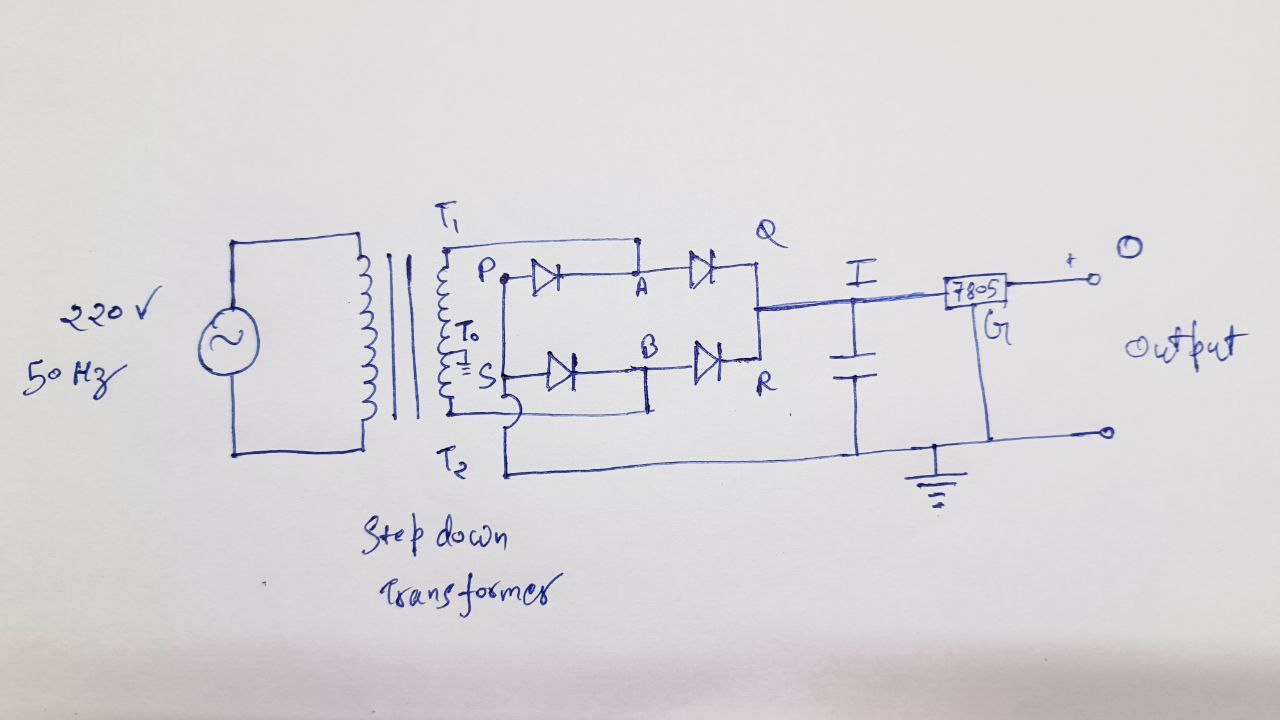
\includegraphics[width=\columnwidth]{figs/circuit.jpg}
    \caption{Schematic diagram of the circuit.}
    \label{fig:ckt}
\end{figure}

\begin{figure}[!htb]
    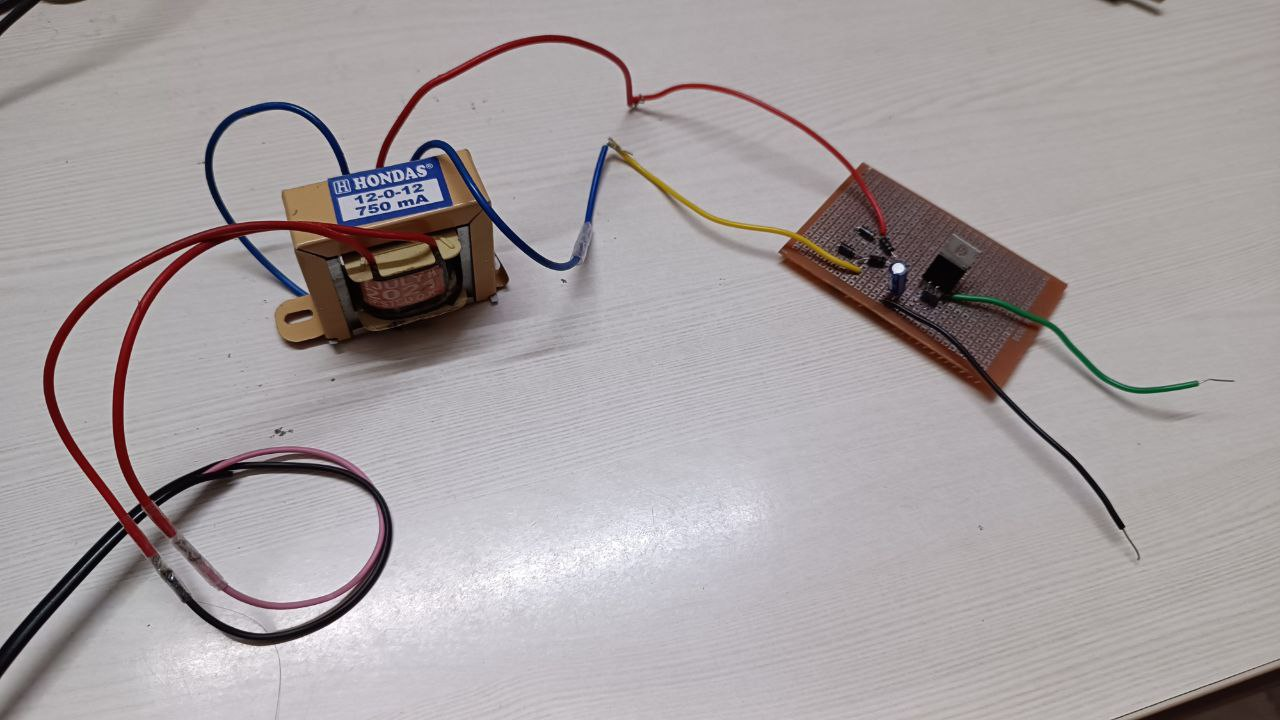
\includegraphics[width=\columnwidth]{figs/Real_pic.jpg}
    \caption{Real picture of the circuit.}
    \label{fig:hardware}
\end{figure}
\subsection{Transformer}
The transformer used is a centre-tapped 12-0-12 step-down 
transformer. The ground and one of the output wires is used
in the charging circuit. The output waveform at this stage is
a 12 V, 50 Hz AC sinusoid.

\subsection{Rectifier}
The full-wave rectifier is realized using four Si diodes arranged in a
bridge form as shown in Fig. \ref{fig:ckt}. The output waveform at this
stage is a DC 12 V, 50 Hz rectified sinusoid.

\subsection{Filter}
This is the main component of the charging circuit. The 100 $mu$F
capacitor acts as a first order analog low pass filter. It filters
around the zero frequency DC component and partially eliminates the
even harmonics associated with the rectified sinusoid. The output 
waveform at this stage consists of the constant DC component. Note
there is no gain and hence we require a regulator to obtain the
required DC 5V supply.

\subsection{Regulator}
The regulator used in this circuit is a 7805 regulator, which outputs
a constant DC supply of 5 V with very little ripple through a 
feedback mechanism. The regulator will work because the DC component 
associated with the rectified waveform is
\begin{align}
    V_{DC} = \frac{2V_p}{\pi} = \frac{2\times12\sqrt{2}}{\pi} > \SI{5}{\V}
\end{align}
where $V_p$ is the peak voltage. Thus, we obtain an almost
constant supply of 5 V DC to charge a mobile phone.

\section{Results}
The screenshots of the waveforms at each stage are shown ahead.

\begin{figure}[!ht]
    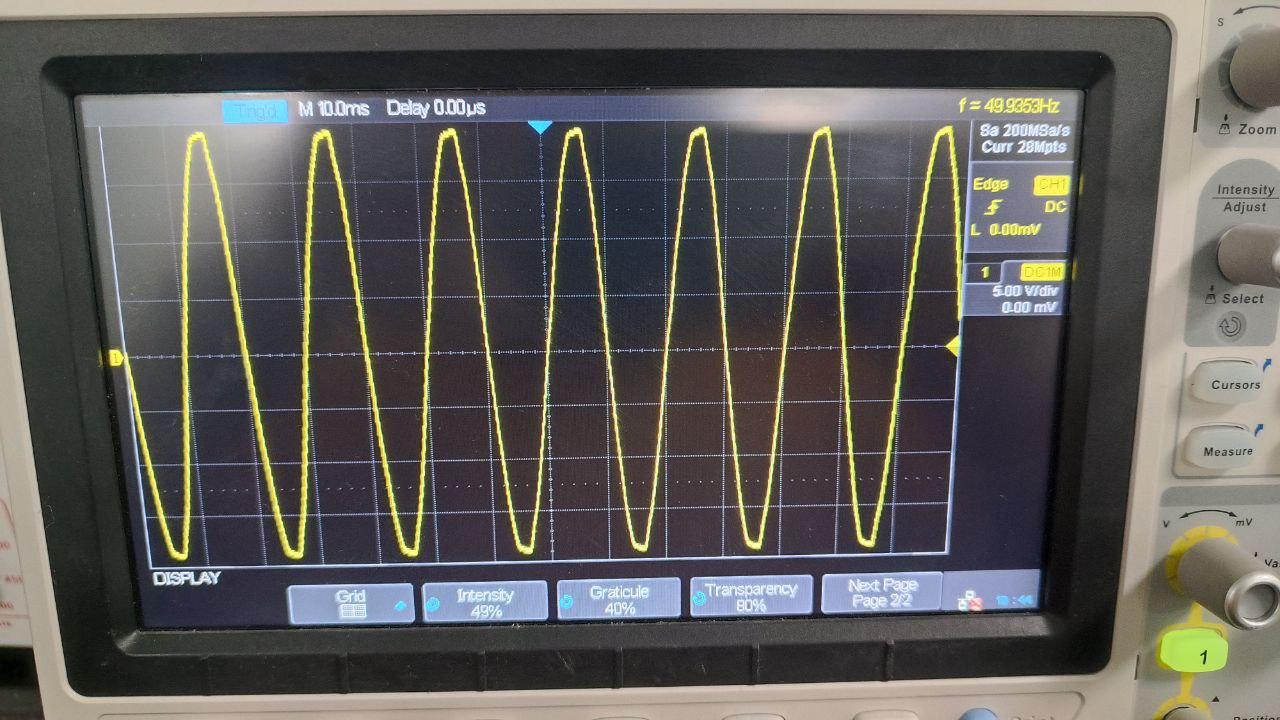
\includegraphics[width=\columnwidth]{figs/figure1.jpg}
    \caption{Output AC waveform at transformer stage across T\textsubscript{1}T\textsubscript{0} (18 V peak).}
    \label{fig:transformer}
\end{figure}

\begin{figure}[!ht]
    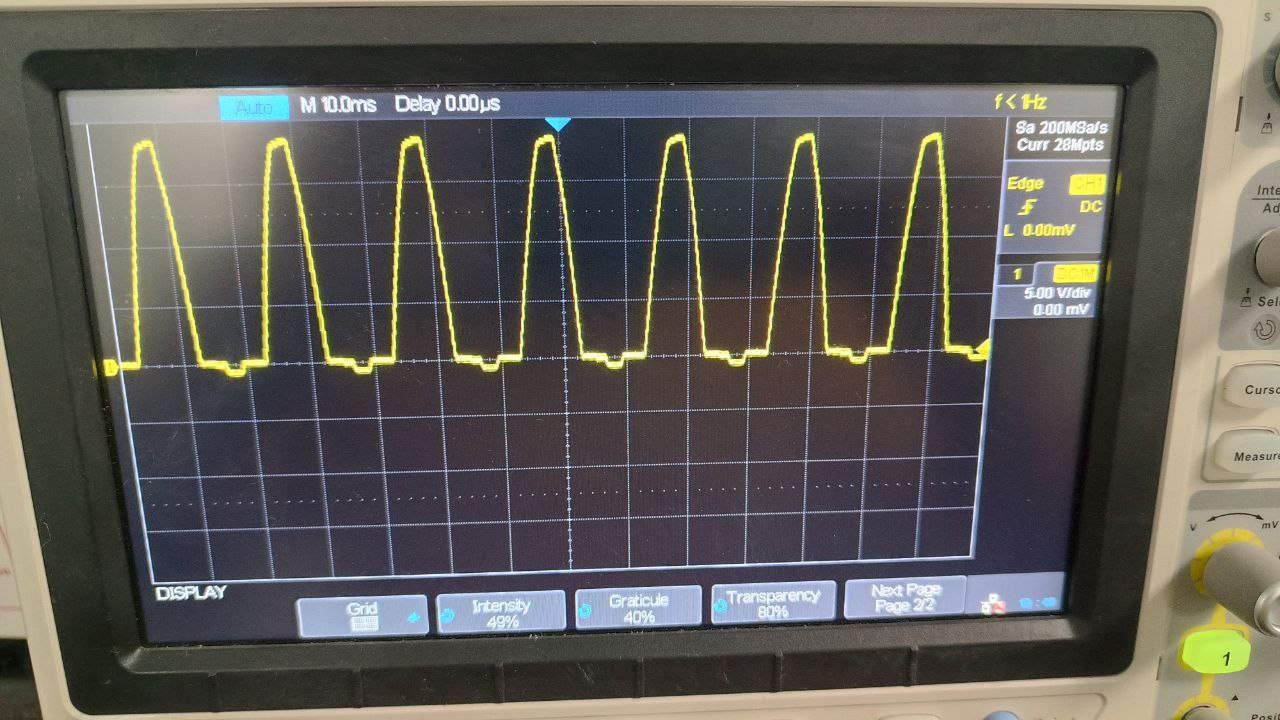
\includegraphics[width=\columnwidth]{figs/figure2.jpg}
    \caption{Output half-wave rectified waveform across diode across AQ (18 V peak).}
    \label{fig:rectifier}
\end{figure}

\begin{figure}[!ht]
    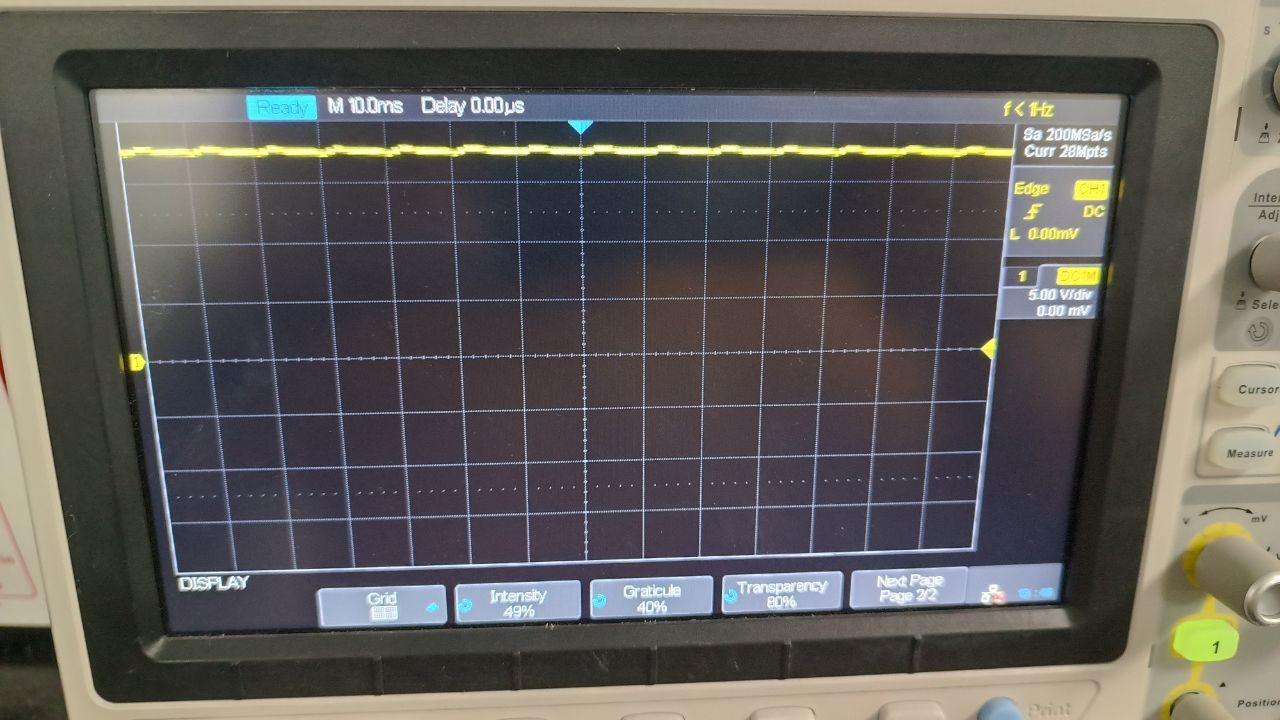
\includegraphics[width=\columnwidth]{figs/figure3.jpg}
    \caption{Output DC waveform at filter stage across IS (18 V).}
    \label{fig:filter}
\end{figure}

\begin{figure}[!ht]
    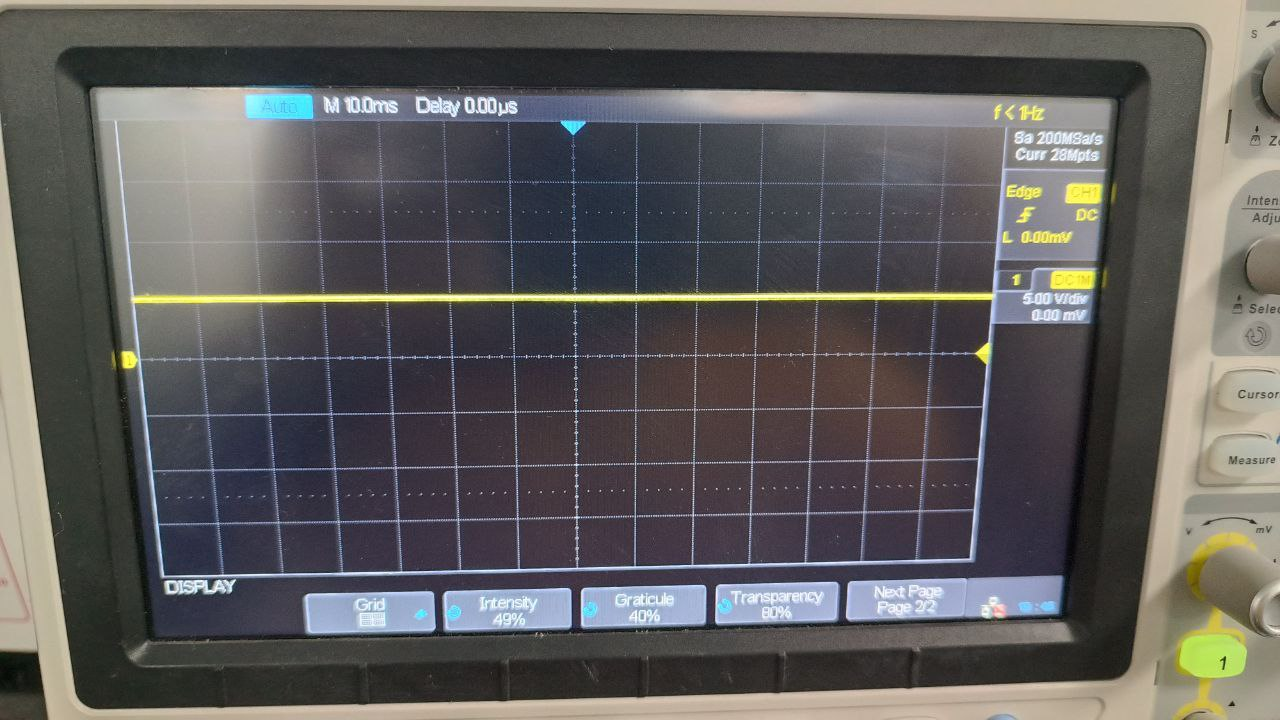
\includegraphics[width=\columnwidth]{figs/figure4.jpg}
    \caption{Output DC waveform at regulator stage across OG (5 V).}
    \label{fig:regulator_dc}
\end{figure}

% \begin{figure}[!ht]
%     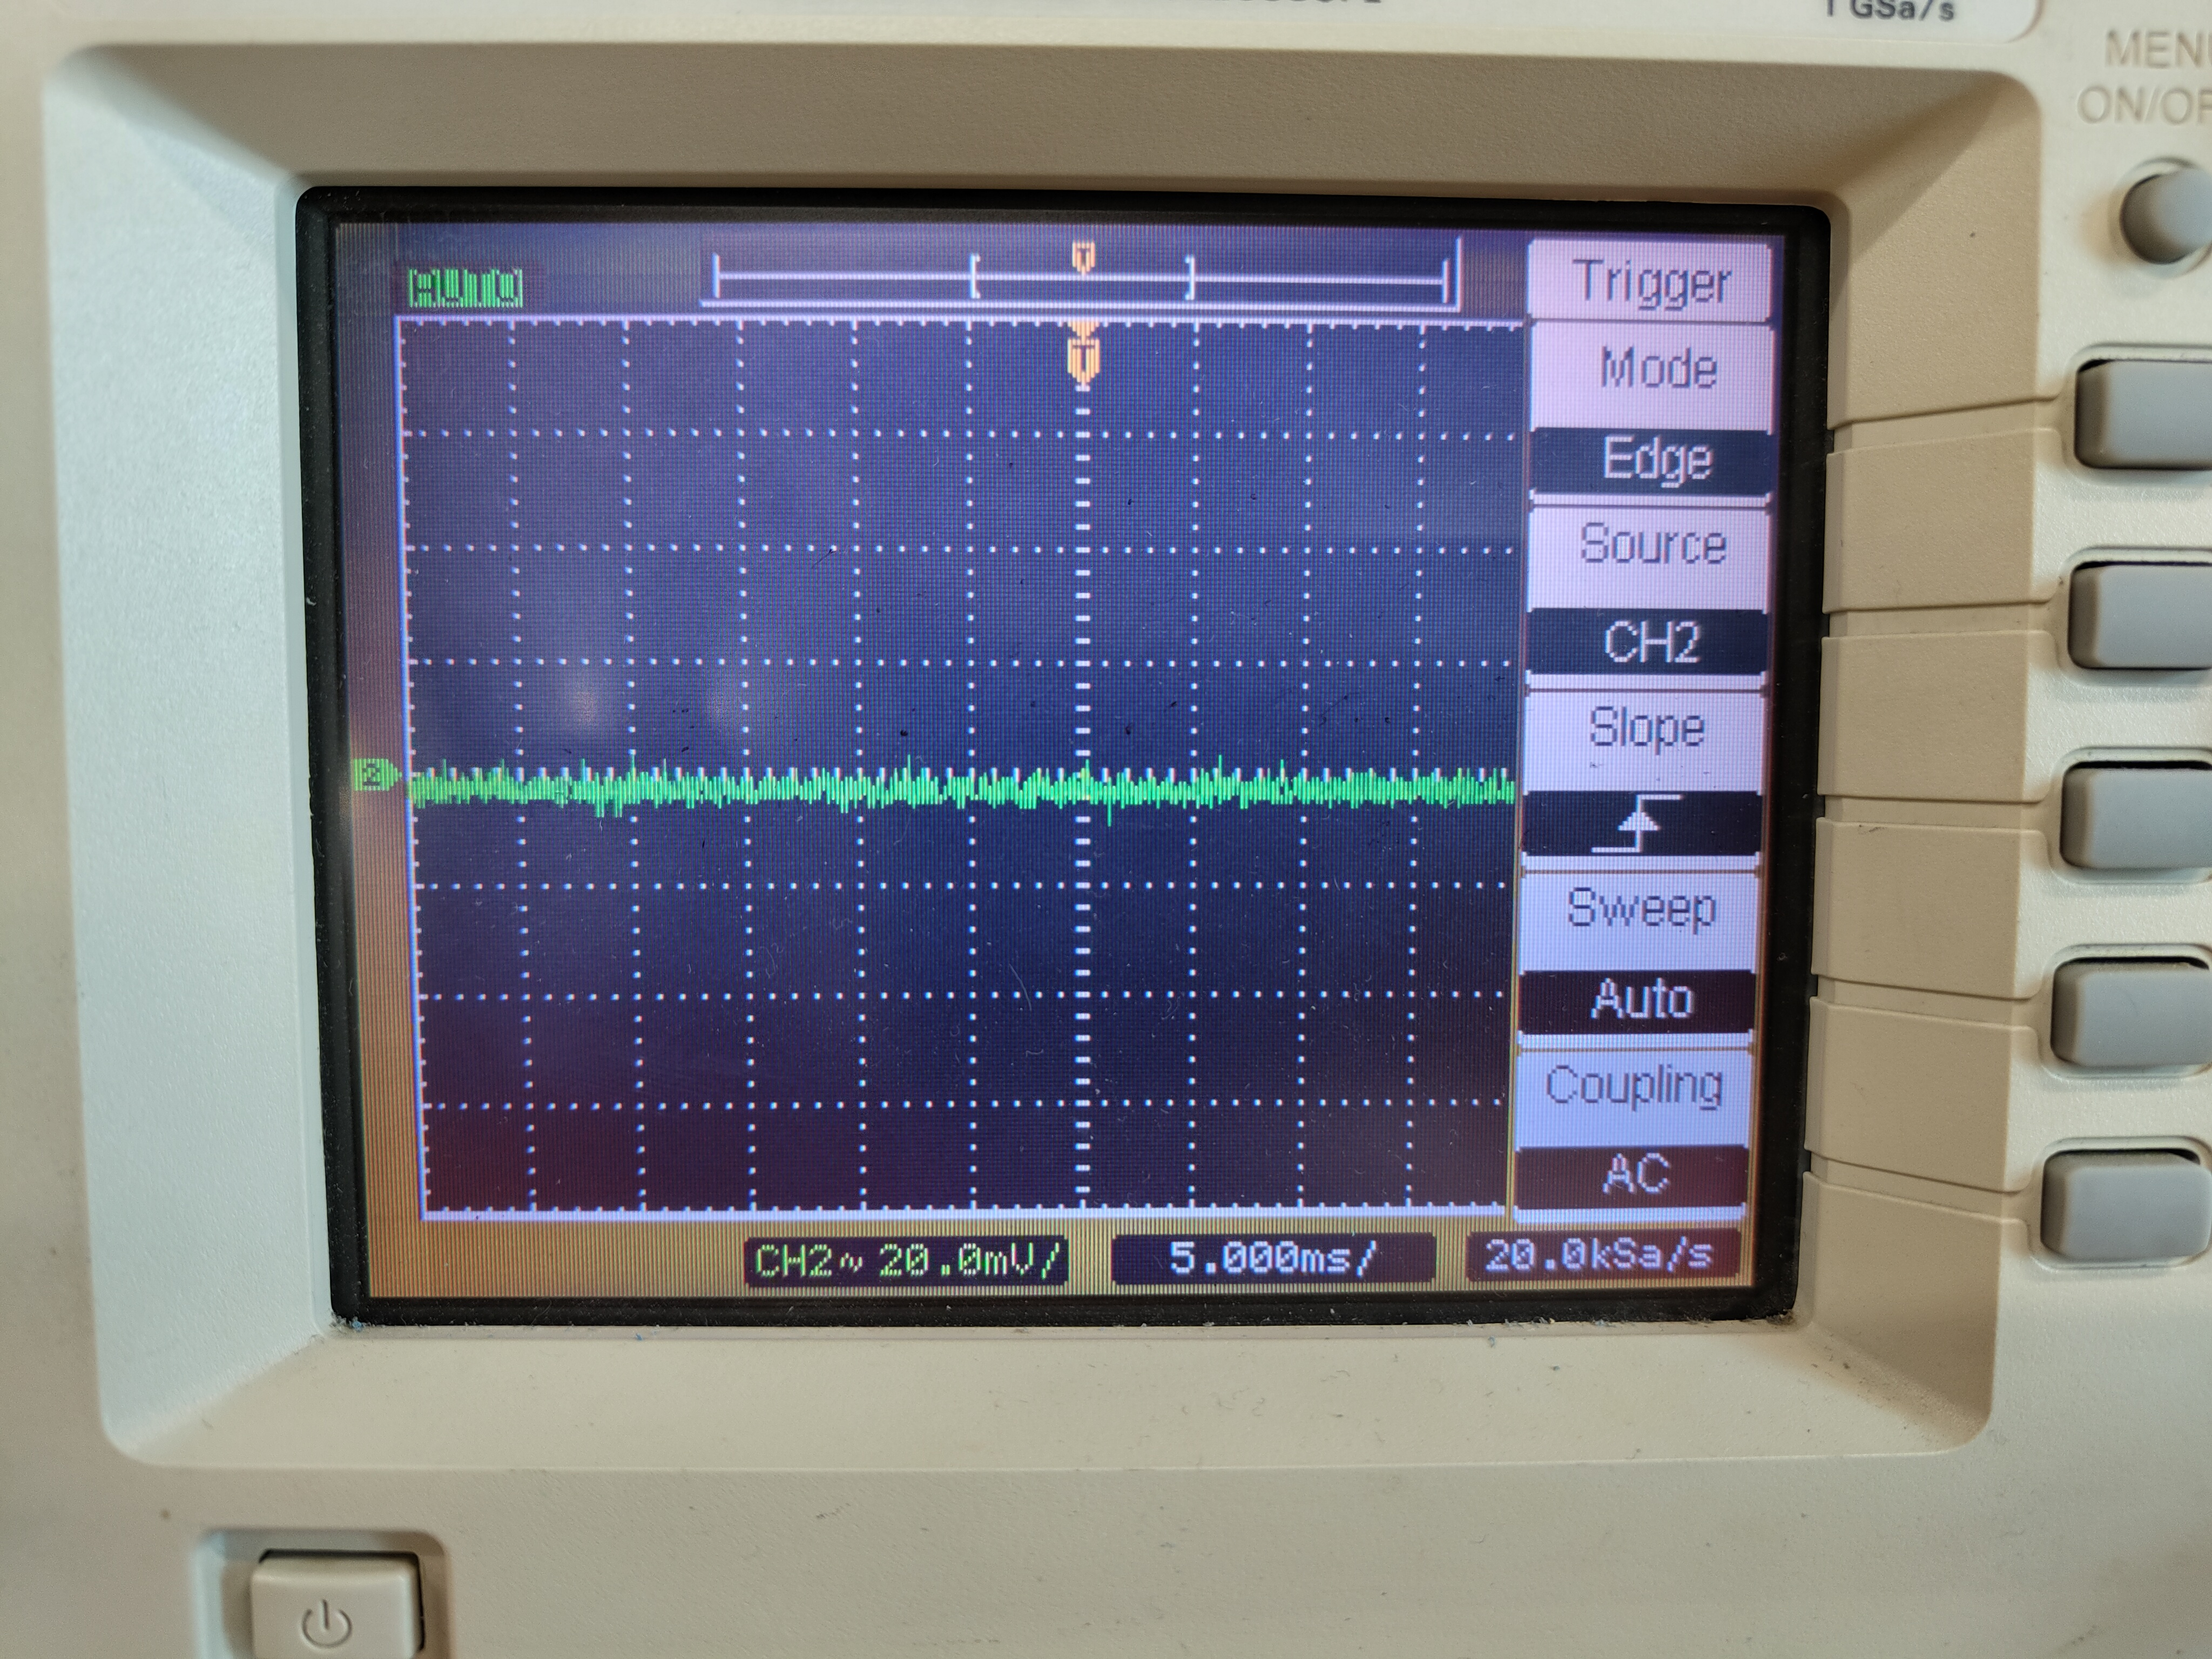
\includegraphics[width=\columnwidth]{figs/regulator_ac.jpg}
%     \caption{Output AC ripple at regulator stage across OG (5 mV).}
%     \label{fig:regulator_ac}
% \end{figure}

\begin{enumerate}
    \item Peak voltage after transformer and rectifier stage, 
        $V_p = \SI[parse-numbers=false]{18}{\V}$.
    \item DC component after filter stage, 
        $V_{DC} = \SI[parse-numbers=false]{18}{\V}$.
    \item DC component after regulator stage, $V_{DC}' = \SI{5}{\V}$.
    % \item Ripple after regulator stage, $\epsilon = \SI{5}{\milli\V}$.
\end{enumerate}

\section{Learning Outcomes}
\begin{enumerate}
    \item Working and implementation of a low-pass analog filter.
    \item Use of regulator to help realise an analog low-pass filter with
        very low cutoff frequency.
    \item Use of lab equipment such as solder, oscilloscope, breadboard, PCB, etc.
        to realize a circuit.
\end{enumerate}
\end{document}
